% !TEX root = main.tex
\chapter{Experimental Results}\label{cha:exp_result}
\section{Setup}\label{sec:setup}
The results in Table~\ref{tab:comp_h} and \ref{tab:comp} reveals, in terms of performance, stability and implementation considerations, two good candidates. The \abbrIRC  as a stand alone control approach and the \abbrRFDC as harmonic cancellation add-on. Due to time limitations, only the harmonic cancellation method was selected to be implemented in this thesis.

The experiments presented in this chapter has been conducted on the rotational stage described in Section~\ref{sec:rotational_stage}. A National Instruments PXI was used to communicate with the crystal collimator and the rotational stage, responsible for acquisition and control. The PXI drives the rotational stage by applying a voltage between [-1, 7.5] V that passes through a linear amplifier with a gain of \unit{20}{\volt/\volt} resulting in an input signal ranging from -20 to 150V. The analogue output has resolution of \unit{10}{\micro\volt}. The linear and the rotational position of the crystal was measured by a (?) and a interferometric system (shown in Figure~\ref{fig:rotationalstage-side}), respectively. The data was acquired by the PXI giving an resolution in linear and rotational position of \unit{?}{\nano\radian} and \unit{?}{\milli\meter}.


\subsection{Implementation}
The control loop consisting of the original controller described in Section~\ref{sec:presentControlApproach} was executed on the PXI with an updating frequency of \unit{2}{\kilo\hertz}. The \abbrRFDC was implemented using LabVIEW and added to the existing control loop. The graphical user interface (\abbrGUI) that was created to operate the cancellation is shown in Figure~\ref{fig:gui}.

\begin{figure}[h]
  \centering %crop: left bottom right top
  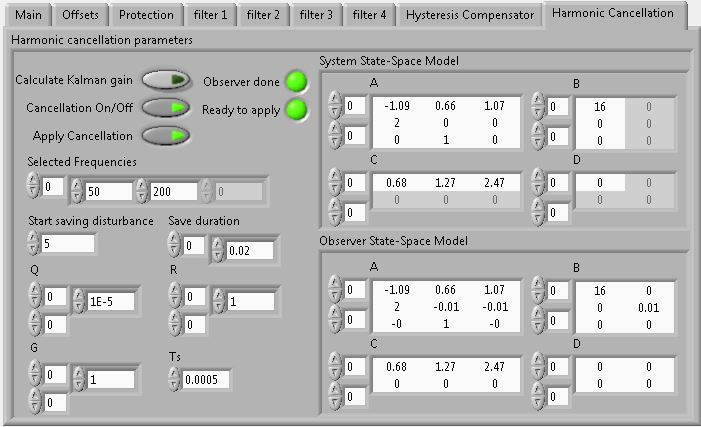
\includegraphics[width=0.8\textwidth]{fig/HC_gui}
  \caption{\label{fig:gui}Graphical user interface of the \abbrRFDC implementation}
\end{figure}

As seen in the \abbrGUI the method requires a system model, specification of the selected frequencies, a time after initialization when the observer shall start and how long it should observe. This time must, for efficient cancellation, be a multiple of the selected disturbance period time. In the initialization phase the observer model is calculated by pressing \emph{Calculate Kalman gain}. The calculations are based on the system model and the specified tuning parameters. Cancellation is initialized by pressing the \emph{Cancellation ON/OFF}, which starts the observation. \emph{Observer done} indicates when the observation has finished and \emph{Ready to apply} when the cancellation is ready to be applied.

\section{Cancellation verification}
Verification of the cancellation effectiveness has been evaluated in a number of different benchmarking test both in open and closed loop. Firstly, single disturbance cancellation was validated by cancelling an artificial disturbance added to the system by a shaker. The shaker consist of a piezoelectric actuator mounted in a prestressed structure, which generates oscillations in symphony with the applied AC voltage. Single disturbance cancellation was also benchmarked with real environmental harmonic disturbances that was not generated by the shaker. Finally the approach was tested for cancellation of multiple frequency components simultaneously.

\subsection{Single disturbance}
The \abbrRFDC was first evaluated in open loop with the aim of cancelling single harmonics generated by the shaker. In the first test the shaker was set to generate an 80Hz disturbance (amplitude set to 300mV). Data was then acquired with and without the disturbance cancellation algorithm active and the result is presented in Figure~\ref{fig:yl_openloop_80} and Figure~\ref{fig:fft_openloop_80} which shows the cancellation performance in time and frequency domain, respectively. Note that the acquisitions were taken successively, in direct contact after one another. The \abbrRFDC attenuates the generated 80Hz signal by 10.7 times. The exact values can be seen in the table to the right of the graph, where the amplitude is presented in linear scale.

\begin{figure}[h]
  \centering %crop: left bottom right top
  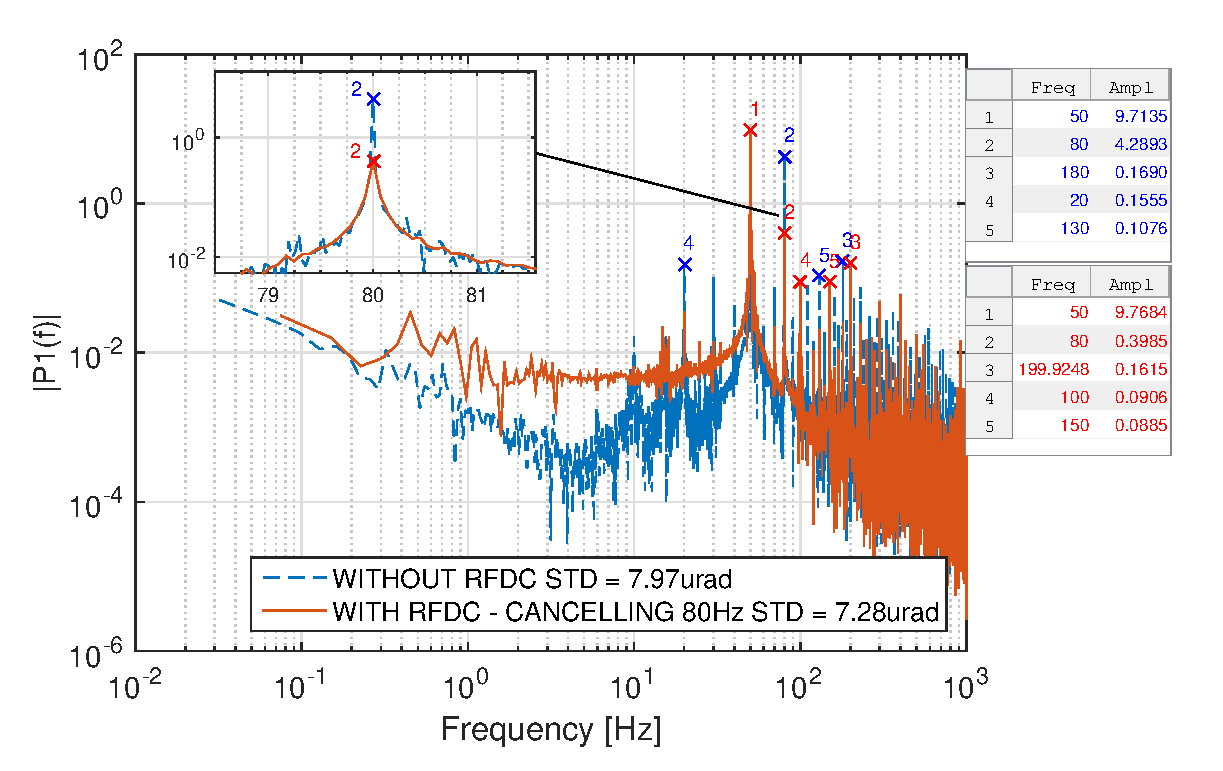
\includegraphics[width=0.85\textwidth]{fig/matlab/fft_openloop_ext_disturbance_80Hz_with_zoom}
  \caption{\label{fig:fft_openloop_80} \abbrFFT of the yaw angle response acquired in open loop with and without the \abbrRFDC active. Cancellation of the 80Hz component generated by the shaker. The table to the right of the figures shows the amplitude of the 5 highest resonance peaks displayed in descending order.}
\end{figure}

Since the disturbance is quite significant with respect to other present peaks, the cancellation can easily be identified by looking in the time domain and the standard deviation of the signal. With the \abbrRFDC active the standard deviation went down from \unit{7.97}{\micro\radian} to \unit{7.28}{\micro\radian}, as shown in Figure~\ref{fig:yl_openloop_80}.

\begin{figure}[h]
  \centering %crop: left bottom right top
  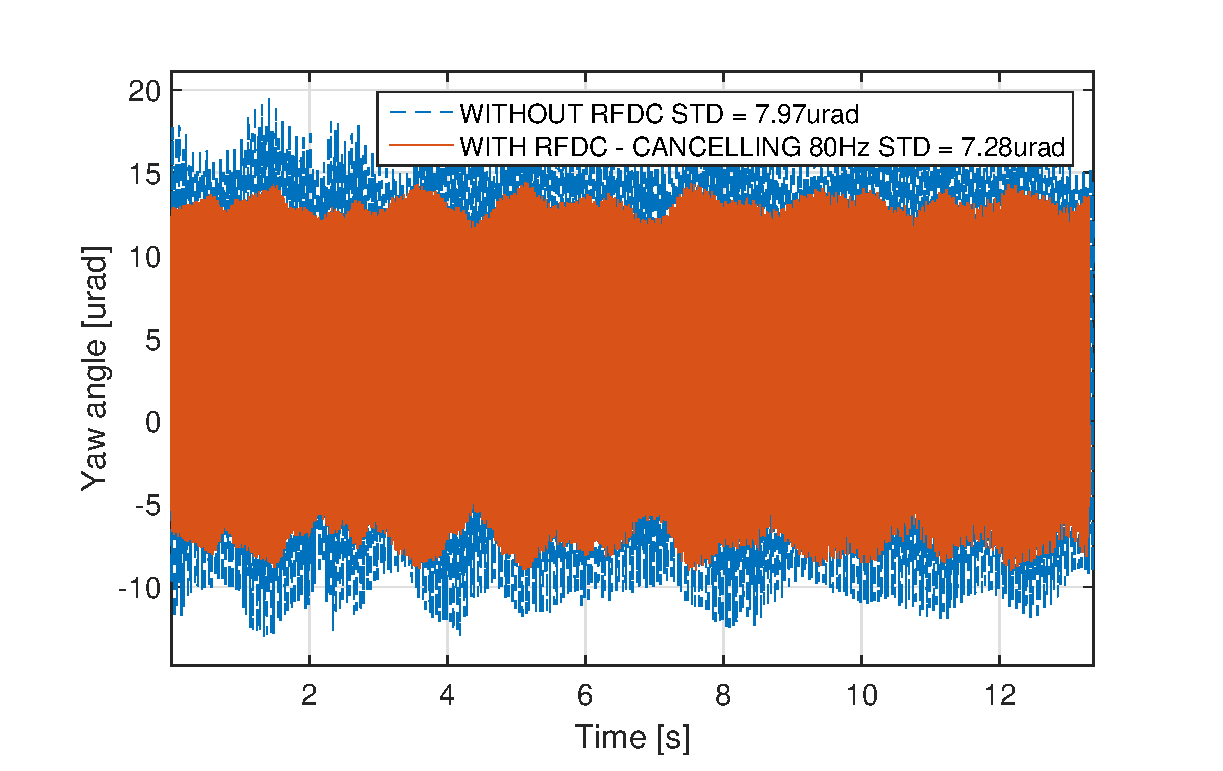
\includegraphics[width=0.8\textwidth]{fig/matlab/yl_openloop_ext_disturbance_80Hz}
  \caption{\label{fig:yl_openloop_80} Open loop response showing the development of the yaw angle over time, with and without the \abbrRFDC active. Cancellation of the 80Hz component generated by the shaker.}
\end{figure}

Similar tests were performed with the controller in closed loop. The performance of the \abbrRFDC is shown in Figure~\ref{fig:fft_closedloop_80}, where the 80Hz resonance peak is attenuated by more than 4 times. The same figure also reveals a small inclination of the yaw angle evolving over time, i.e. the attenuation loses effect. In fact, looking over a larger period of time, the effect is oscillating. This effect is known as the "beat effect" and discussed further in Section~\ref{subsec:longterm}.

\begin{figure}[h]
  \centering %crop: left bottom right top
  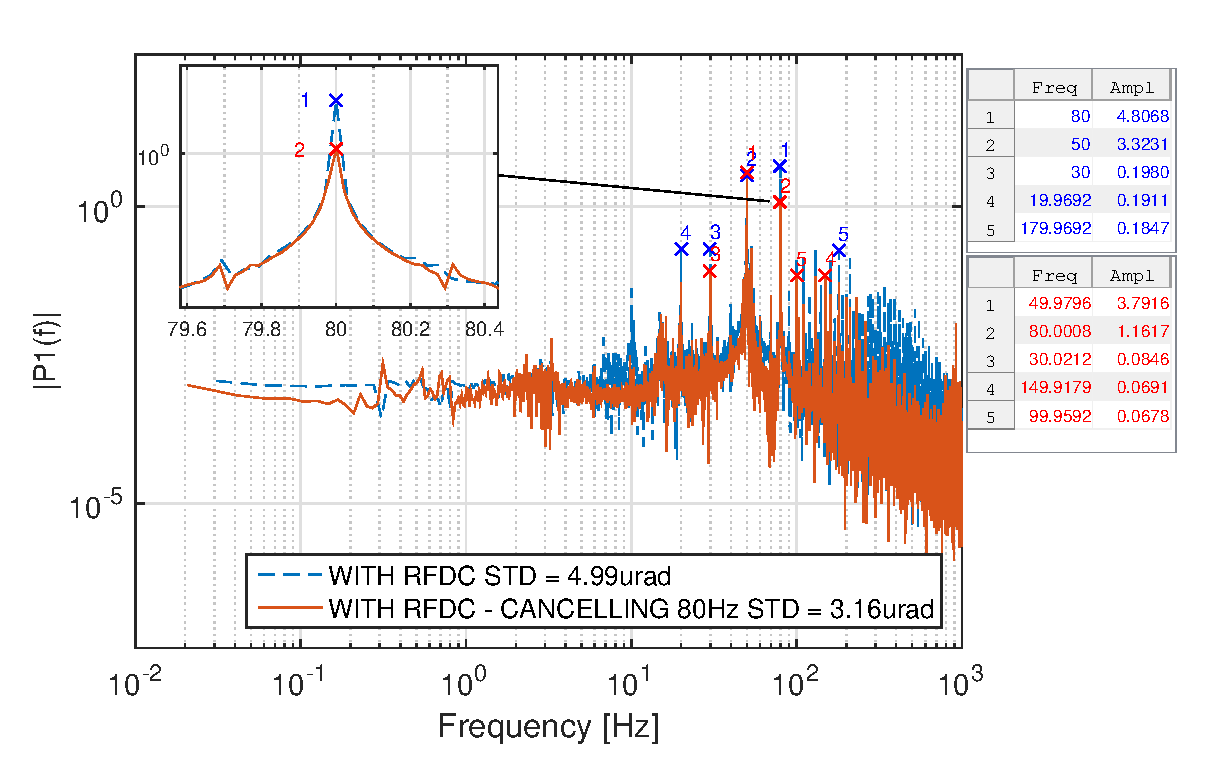
\includegraphics[width=0.85\textwidth]{fig/matlab/fft_closedloop_ext_disturbance_80Hz_with_zoom_2}
  \caption{\label{fig:fft_closedloop_80} \abbrFFT of the yaw angle response acquired in closed loop with and without the \abbrRFDC active. Cancellation of the 80Hz component generated by the shaker.}
\end{figure}

\begin{figure}[h]
  \centering %crop: left bottom right top
  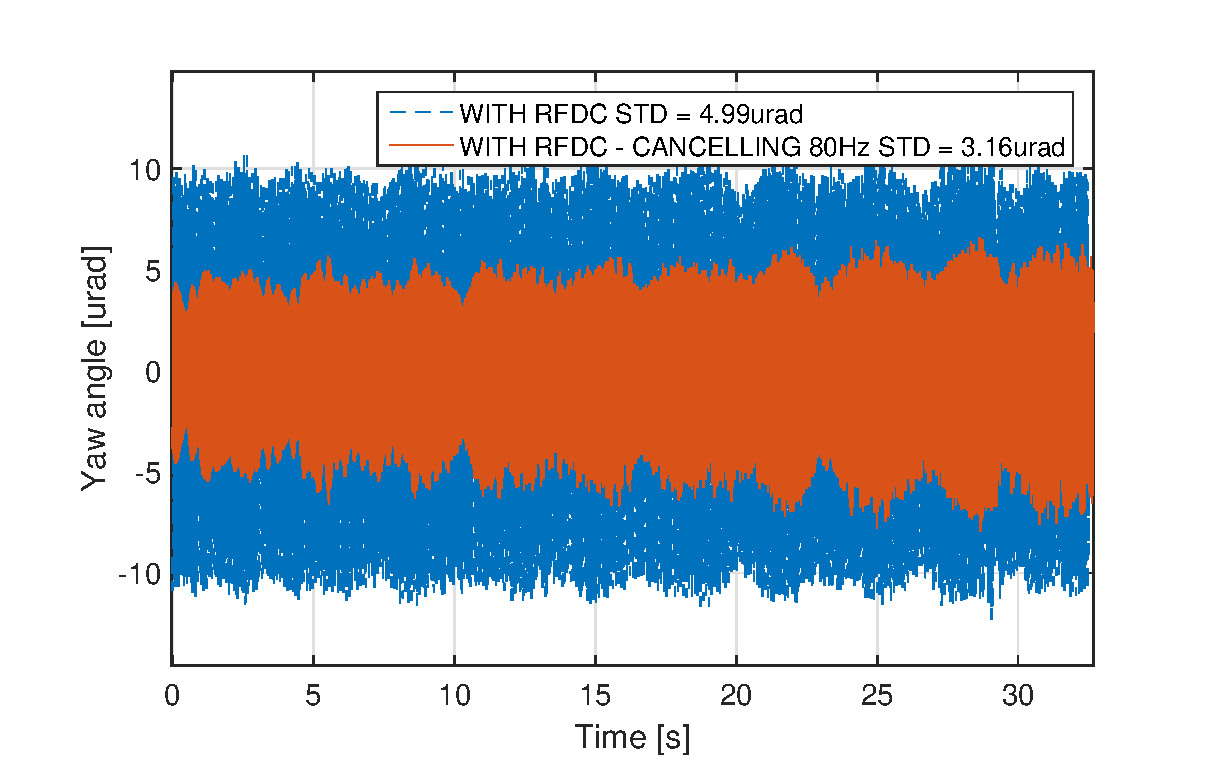
\includegraphics[width=0.8\textwidth]{fig/matlab/yl_closedloop_ext_disturbance_80Hz_2}
  \caption{\label{fig:yl_closedloop_80} Closed loop response showing the development of the yaw angle over time, with and without the \abbrRFDC active. Cancellation of the 80Hz component generated by the shaker.}
\end{figure}

To further verify the performance, similar tests were also performed without the shaker applying an external disturbance. The selected disturbance was now identified by taking closed loop measurements to find dominating frequencies not attenuated by the controller itself. The 50Hz was identified to be the most dominating component as shown in the series without the \abbrRFDC active in Figure~\ref{fig:fft_closedloop_50}. This frequency was selected and attenuated by more than 2 times with \abbrRFDC active, as presented in the same figure.

\begin{figure}[h]
  \centering %crop: left bottom right top
  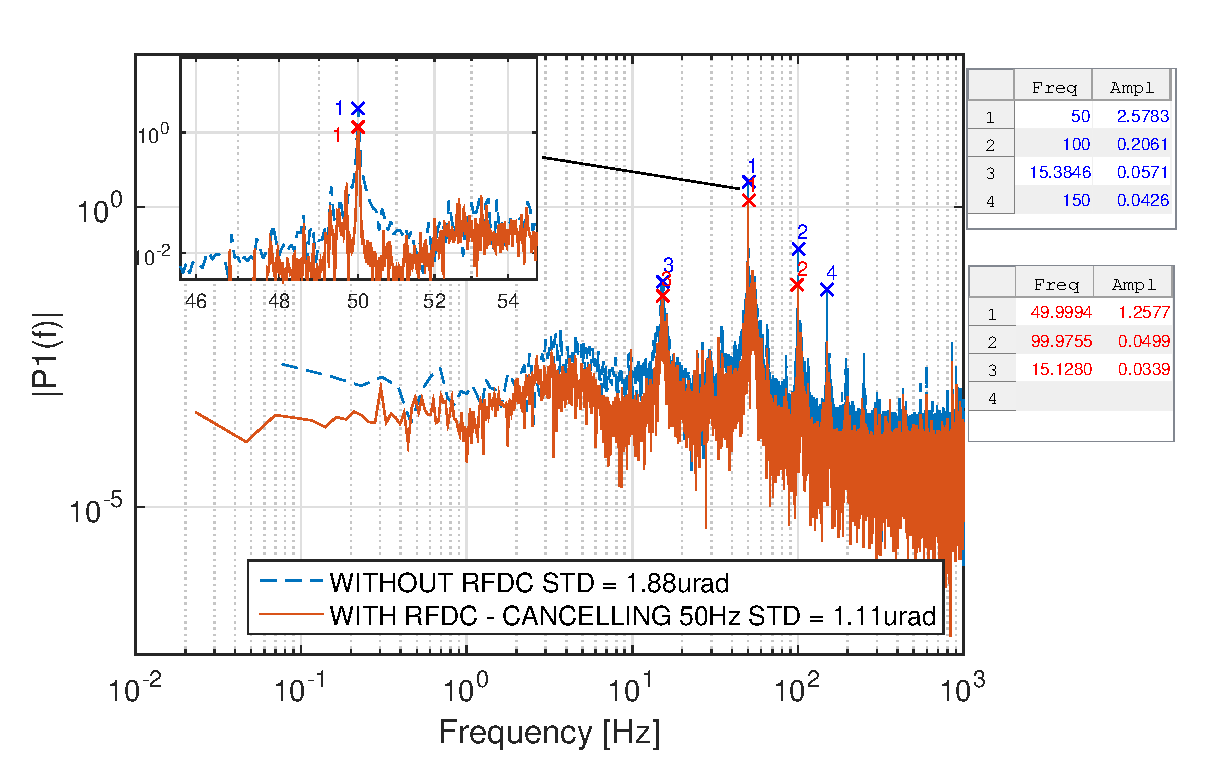
\includegraphics[width=0.85\textwidth]{fig/matlab/fft_closedloop_50Hz}
  \caption{\label{fig:fft_closedloop_50}\abbrFFT of the yaw angle response acquired in closed loop with and without the \abbrRFDC active. Cancellation of the 50Hz component originating from environmental disturbances.}
\end{figure}

The attenuation of the 50Hz component improved the overall yaw angle accuracy as shown in Figure~\ref{fig:transient_closedloop_50}, where the activation transient is captured.
\FloatBarrier
\begin{figure}[h]
  \centering %crop: left bottom right top
  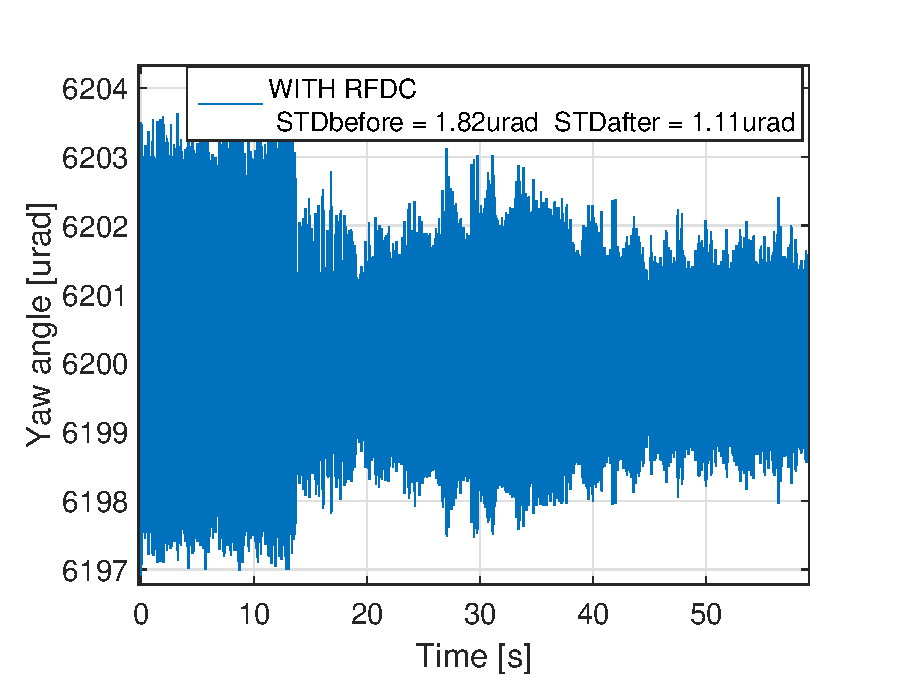
\includegraphics[width=0.8\textwidth]{fig/matlab/transient_closedloop_50Hz}
  \caption{\label{fig:transient_closedloop_50}Closed loop transient showing the response of the activation of the \abbrRFDC. Cancellation of the 50Hz component originating from environmental disturbances.}
\end{figure}


\subsection{Multiple disturbances}
The cancellation of several disturbances simultaneously was verified by trying to cancel out a 50Hz component originating from environmental disturbances in the laboratory and a 80 Hz generated by the shaker. Figure~\ref{fig:mult5080} shows the \abbrFFT of the first 10 seconds before and after the cancellation is applied. More data was acquired during the measurement but since the the system suffers from the "beat effect" only the first 10 seconds were picked out in order to show the controller ability. During this period of time the 50Hz component is suppressed by more than 4 times and the 80Hz component by more than 2.8 times as seen in the figure and its corresponding tables.

The aim of the \abbrRFDC is to have the ability to select specific frequencies. Since the 50Hz component is the most dominating disturbance in the system, one could expect that when the 50Hz is suppressed efficiently, also several other components might be attenuated. To prove that the \abbrRFDC has this capability of canceling frequencies without affecting others, another test was performed only canceling the 50Hz component. The result can be seen in Figure~\ref{fig:mult50no80}, where it is obvious that the 80Hz component is not affected by the cancellation of the 50.

\begin{figure}[h]
  \centering %crop: left bottom right top
  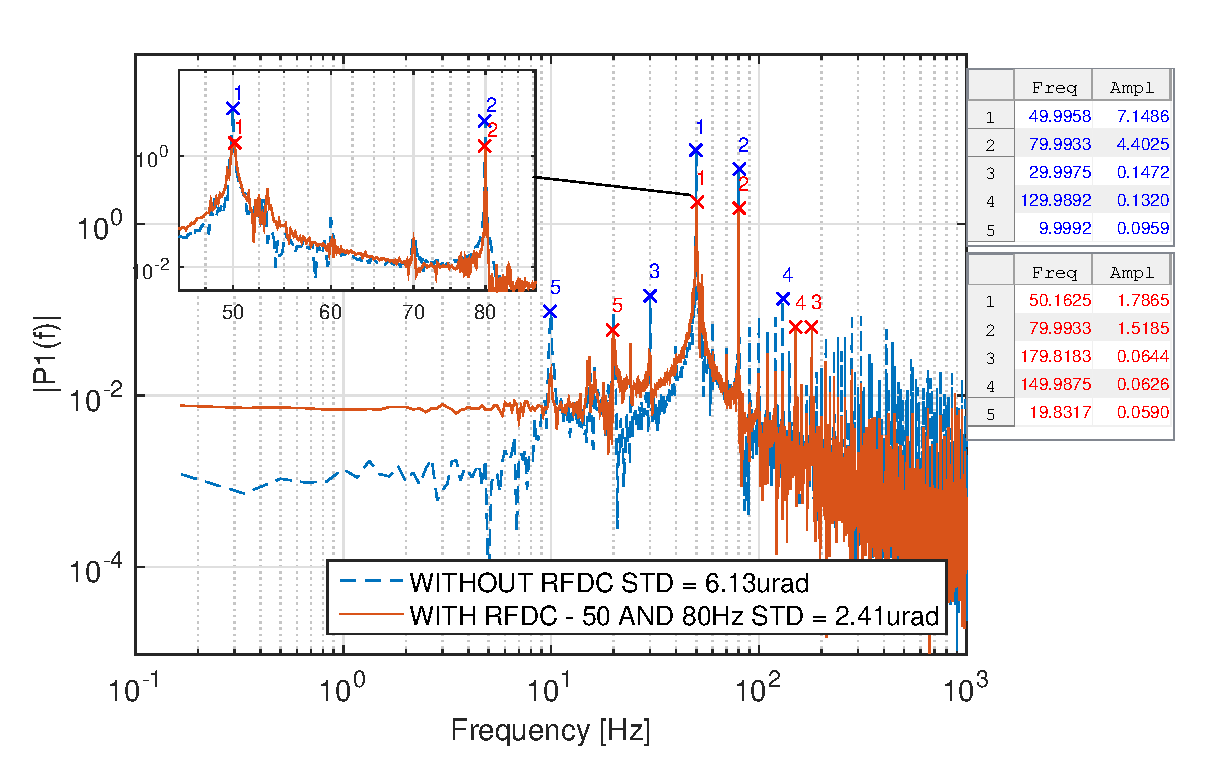
\includegraphics[width=1\textwidth]{fig/matlab/mult_50_80_closed_loop}
  \caption{\label{fig:mult5080} Multiple cancellation in closed loop of the 50 and the 80Hz component. The plot is based on a 10s long acquisition.}
\end{figure}

\begin{figure}[h]
  \centering %crop: left bottom right top
  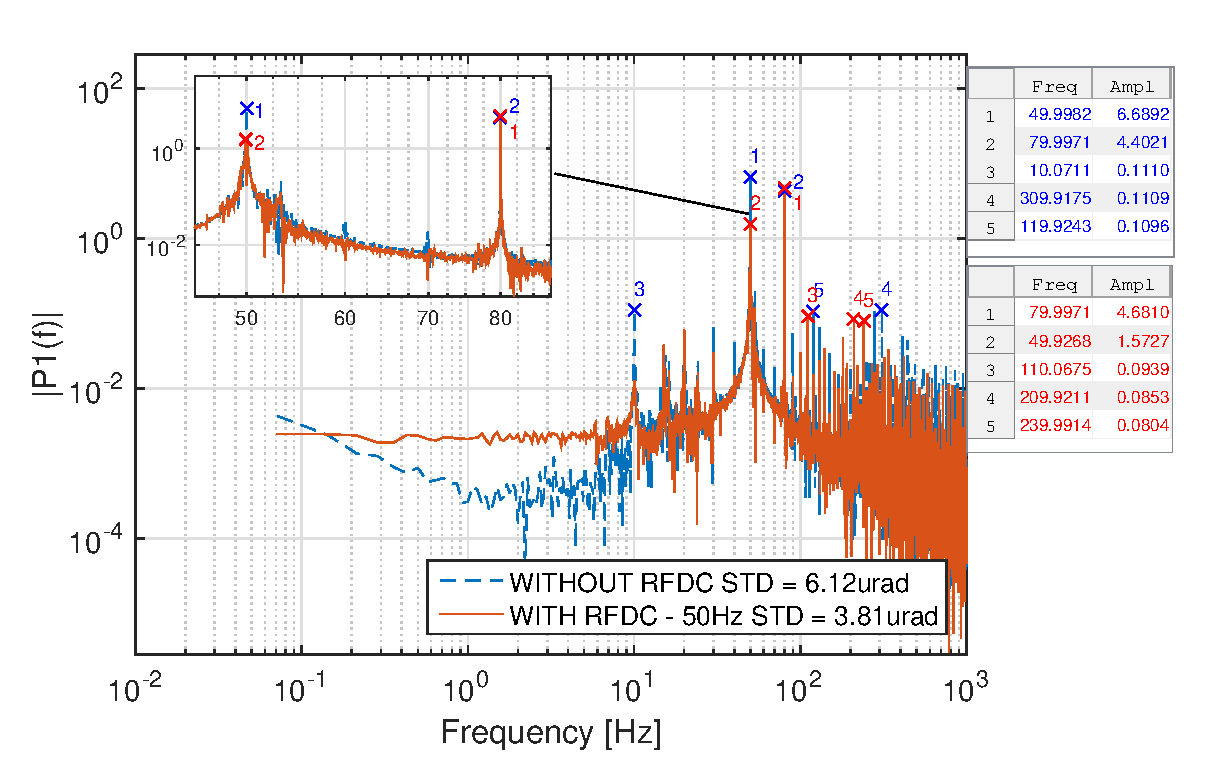
\includegraphics[width=1\textwidth]{fig/matlab/mult_50_selected_closed_loop}
  \caption{\label{fig:mult50no80} Cancellation in closed loop of the 50Hz without affecting the 80Hz component.The plot is based on a 10s long acquisition.}
\end{figure}

\FloatBarrier
\subsection{General findings}\label{subsec:longterm}
The capturing time, should if possible, be kept as low as possible in order to prevent modeling low frequency behavior. For low frequency disturbance cancellation, a bandpass filter should be considered to be included. Figure~\ref{fig:bandpass_imp} shows the \abbrFFT of the replicated disturbance signal. Optimally this should solely contain the selected frequency and no other components, but as seen in (a) this is not the real case. The effect of an inclusion of a bandpass filter is shown in (b), where the 15 Hz components is filtered out from the other low frequency components. The filter is designed with care to keep zero phase shift for 15Hz components. However, this filter includes phase shift for all other components including the 50Hz which has shown to imply in a worsened overall tracking accuracy.

\begin{figure}[h!]
  \centering %crop: left bottom right top
  \subfloat[][Without bandpass filter]{
  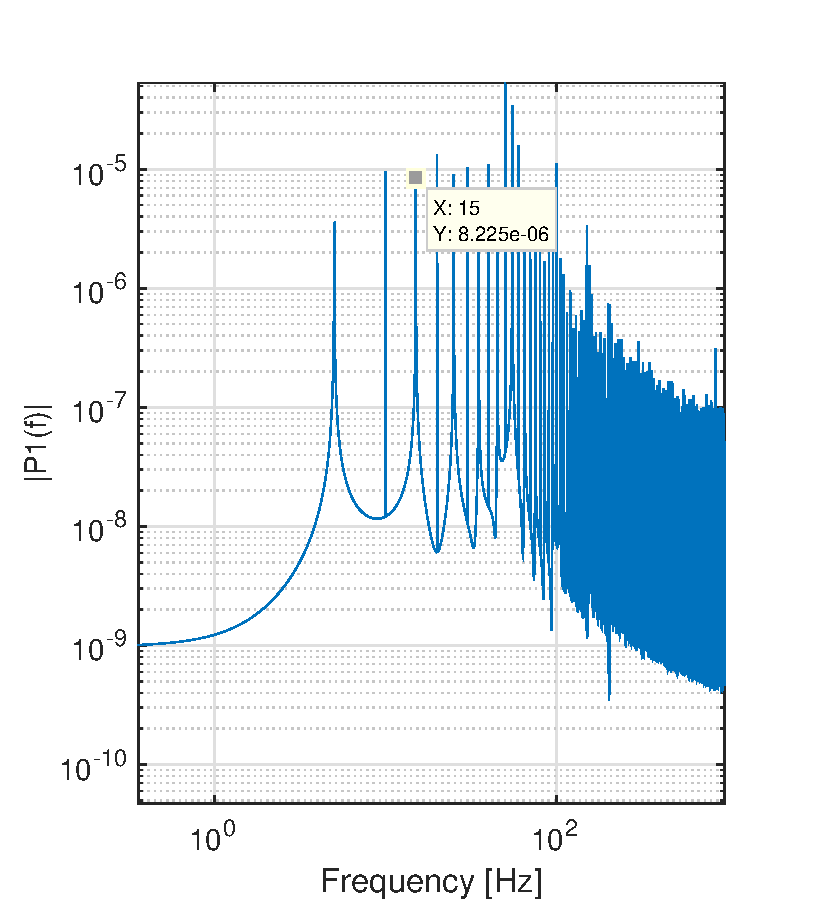
\includegraphics[width=0.46\textwidth, trim=0cm 0cm 0.8cm 0cm, clip=true]{fig/matlab/effect_of_bandpass}}
  \qquad
  \subfloat[][With bandpass filter]{
  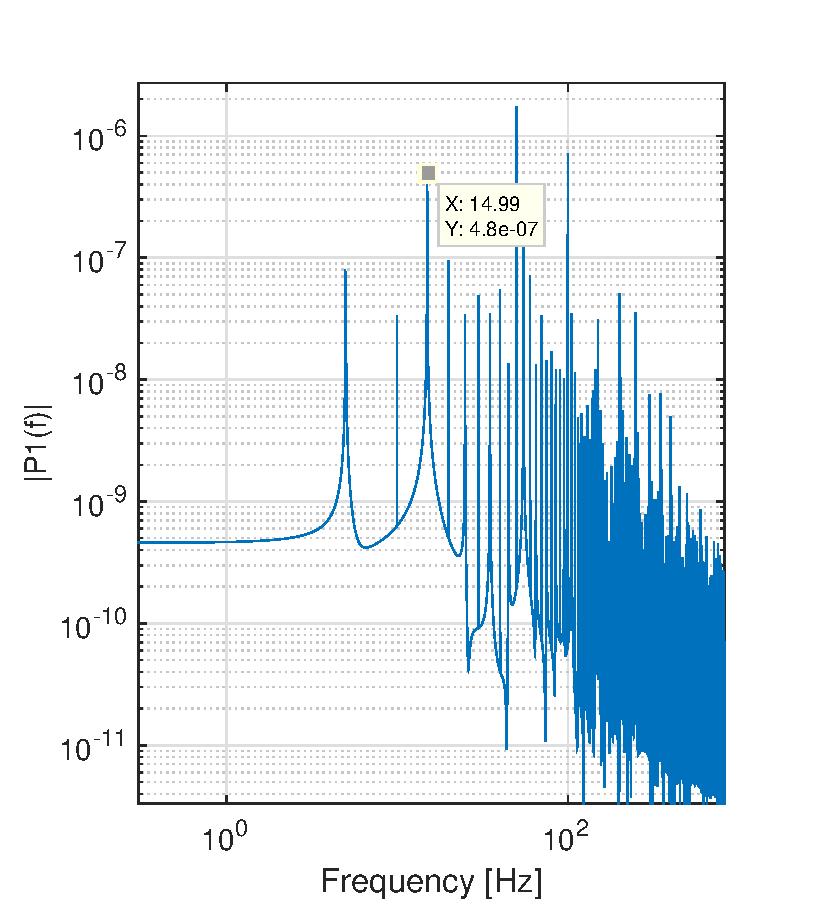
\includegraphics[width=0.46\textwidth, trim=0cm 0cm 0.8cm 0cm, clip=true]{fig/matlab/effect_of_bandpass2}}
  \caption{\label{fig:bandpass_imp} \abbrFFT of the observed signal where (a) shows the signal before and (b) after the filter.}
\end{figure}
\FloatBarrier
During the measurements, an oscillating effect in the performance cancellation was observed known as the "beat effect", explained in Section~\ref{subsec:beat}. The effect is clearly visible in Figure~\ref{fig:beateffect}, where the 50Hz component is only canceled a fraction of the total acquisition time. According to the theory, the envelope should have half the difference between the two frequencies. The envelope in Figure~\ref{fig:beateffect} has a period of 50 seconds giving a 0.04 Hz difference in frequency between the two signals.

To verify that the beat effect was not induced by the algorithm itself, a simple test with 2 artificial disturbances were performed. The two disturbances where created and injected directly in the program on the input that was fed via the amplifier to the rotational stage. These frequencies were then set to be canceled by the \abbrRFDC, using the observed disturbances on the output. The result is shown in Figure~\ref{fig:nobeat}, where the std of the yaw angle displacement can be seen with and without cancellation. The cancellation is here kept constant over 2 minutes, showing no sign of the beat effect.

\begin{figure}[h!]
  \centering %crop: left bottom right top
  \subfloat[][Yaw angle displacement]{
  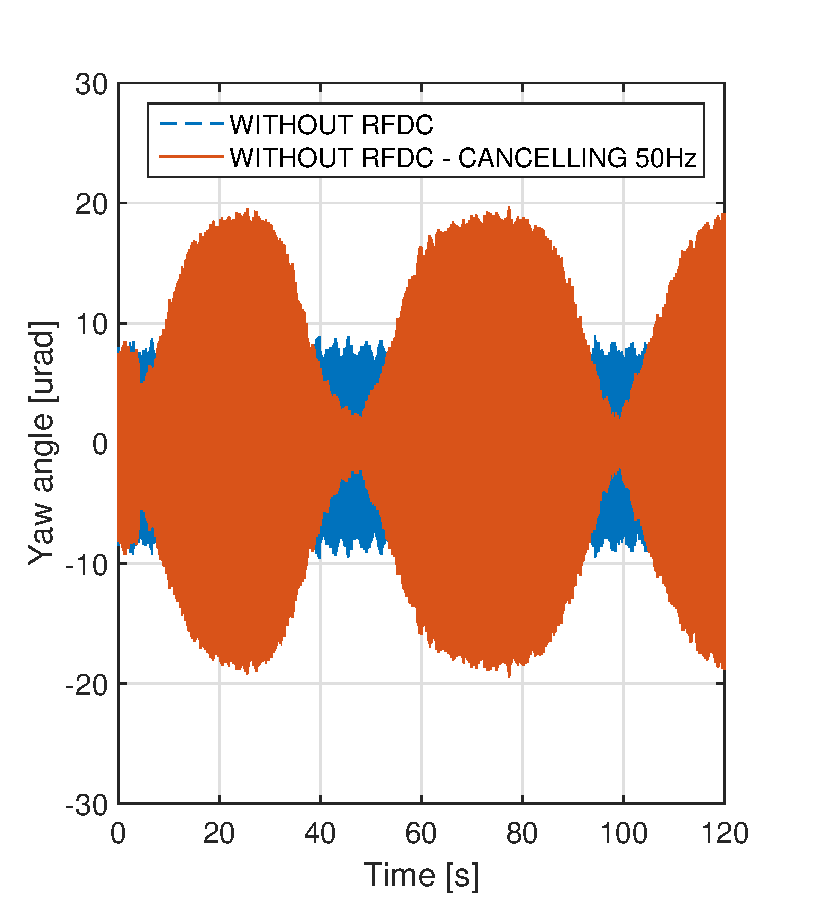
\includegraphics[width=0.46\textwidth, trim=0cm 0cm 0.8cm 1cm, clip=true]{fig/matlab/beat_effect_yl}}
  \qquad
  \subfloat[][Std of the yaw angle displacement]{
  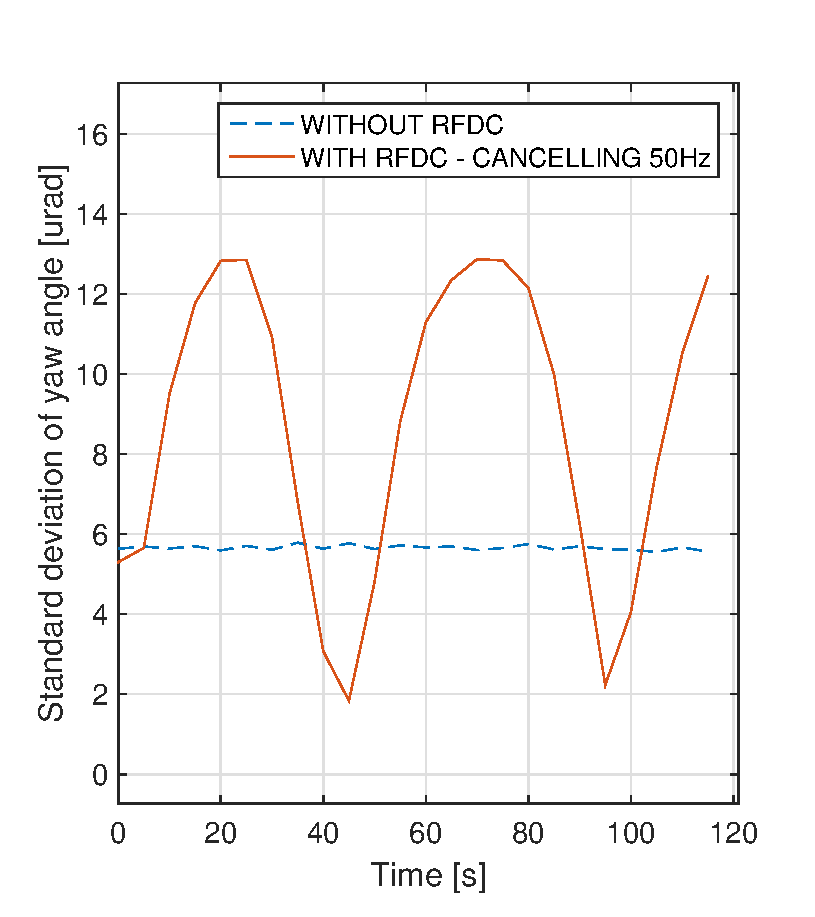
\includegraphics[width=0.46\textwidth, trim=0cm 0cm 0.8cm 1cm, clip=true]{fig/matlab/beat_effect}}
  \caption{\label{fig:beateffect} Cancellation performance of the 50Hz component suffering from the beat effect. The standard deviation taken as an average of (a) every 5 seconds is shown in (b).}
\end{figure}

\begin{figure}[h!]
  \centering %crop: left bottom right top
  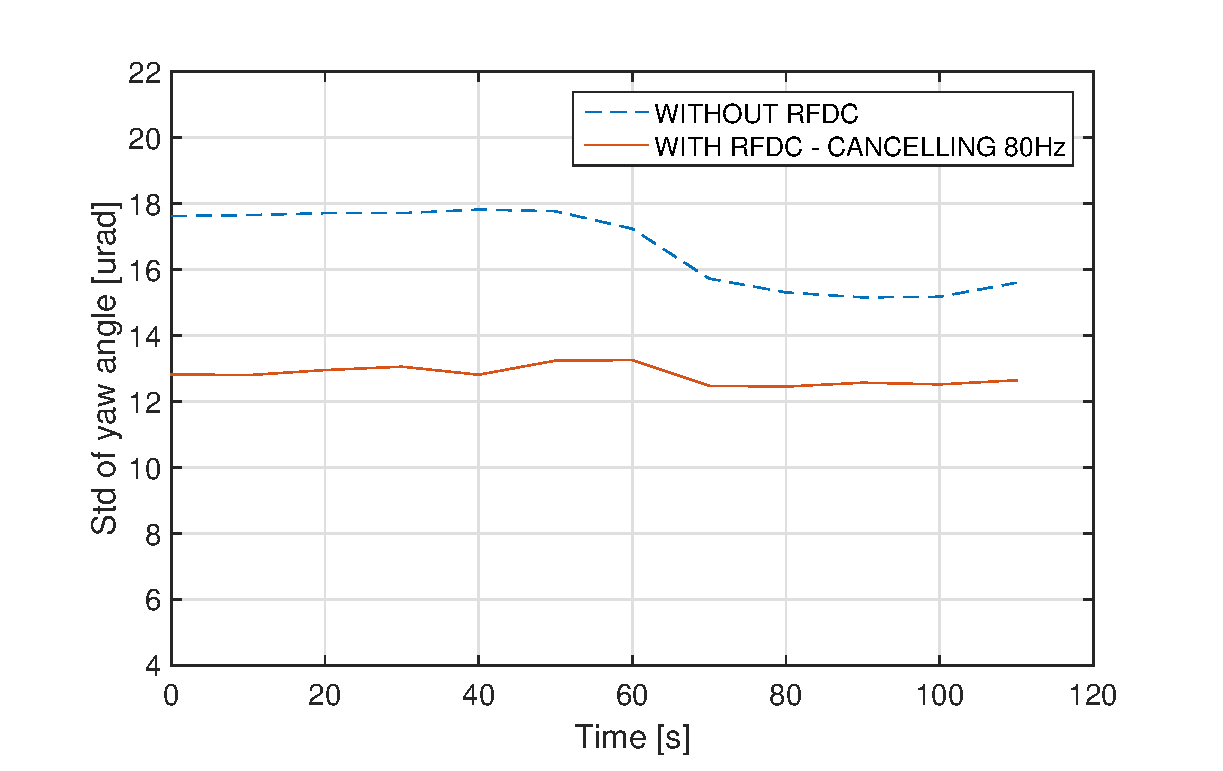
\includegraphics[width=0.8\textwidth, trim=0cm 0cm 0cm 0cm, clip=true]{fig/matlab/no_beat_effect_dist_injected_programatically}
  \caption{\label{fig:nobeat}Cancellation of artificial disturbances not suffering from the beat effect.}
\end{figure}
